% ================================================================
% The printable version of latex/starters/targeted/KS3/algebra/expandingDoubleBracketsStarter.tex
%
% This is the same deck, laid out to be handed out rather than put on
% the board. Every slide is shown as it stands before any answer is
% revealed, and 4 copies of it go on one page of A4, two by two, so
% that a printed page cuts into four question sheets.
%
% Every slide of the deck is here, the title page included, and each takes
% exactly one page. So page 1 is the first slide, page 2 the second, and
% printing the pages you want is how you print the starters you want.
%
%   made from           latex/starters/targeted/KS3/algebra/expandingDoubleBracketsStarter.tex
%   pages on the sheet  4, one per slide of the deck
%   copies of each      4, two by two on A4 landscape
%   printing rules      version 3
%
% Nothing was reworded, nothing was rewritten and nothing was left out.
% Each slide is the slide from the deck, asked for at its first step,
% which is how the answers stay hidden.
%
% Please don't edit this file. It is written again from the one it was
% made from whenever that changes, so an edit here would be lost - edit
% that file instead and this one follows.
% ================================================================
\documentclass{beamer}
\usetheme{default} % You can swap theme if you like (e.g., Madrid, Boadilla)
\usepackage{tikz} 

% ================================================================
% Answer-overlay helpers
% ================================================================
\newcommand{\ablank}[1]{%
  \alt<2>{\textcolor{red}{#1}}{\underline{\phantom{#1}}}%
}
\newcommand{\ashow}[1]{\uncover<2->{\textcolor{red}{\small #1}}}
\newcommand{\ashowq}[1]{\alt<2->{\textcolor{red}{\small #1}}{?}}

% Answers drawn straight on to a TikZ diagram, revealed on overlay 2 like \ashow.
% Space is reserved on overlay 1, so the diagram does not move between slides.
\usetikzlibrary{overlay-beamer-styles}
\tikzset{
  ans/.style     = {red, thick, visible on=<2->},
  ansfill/.style = {red!15, visible on=<2->},
  anslab/.style  = {red, font=\tiny, visible on=<2->},
}

\title{Starter: Expanding Brackets}
\author{Year 8}
\date{}

% ---------------------------------------------------------------
% Added so this deck prints four slides to a page. Nothing above
% this line was changed.
% ---------------------------------------------------------------
\usepackage{pgfpages}

% 4 slides to a sheet of A4, two by two, with a thin line round each
% so that the page can be cut up.
%
% Each slide keeps a margin of 1mm around it and no more, so the four fill
% the sheet and the pieces they cut into are as big as the paper allows. Only
% one direction actually comes out that tight: a slide is a different shape
% from a quarter of a sheet of A4, so it is scaled to fit and the slack it
% cannot use is left along whichever pair of edges it did not fill.
\pgfpagesuselayout{4 on 1}[a4paper,landscape,border shrink=1mm]
\pgfpageslogicalpageoptions{1}{border code=\pgfusepath{stroke}}
\pgfpageslogicalpageoptions{2}{border code=\pgfusepath{stroke}}
\pgfpageslogicalpageoptions{3}{border code=\pgfusepath{stroke}}
\pgfpageslogicalpageoptions{4}{border code=\pgfusepath{stroke}}

% There is nothing on paper to click, and a slide announcing a new section
% would sit between two copies of the same question and put every page after
% it out of step with the grid.
\setbeamertemplate{navigation symbols}{}
\AtBeginPart{}
\AtBeginSection{}
\AtBeginSubsection{}
\AtBeginSubsubsection{}
\begin{document}

\begin{frame}<1>
  \titlepage
\end{frame}
\begin{frame}<1>
  \titlepage
\end{frame}
\begin{frame}<1>
  \titlepage
\end{frame}
\begin{frame}<1>
  \titlepage
\end{frame}

% ---------- STARTER (2x2 layout) ----------
\begin{frame}<1>{Starter: Expand each expression}
% Option A: simple 2x2 grid using minipages (consistent spacing)
\begin{minipage}[t]{0.48\textwidth}
  \begin{block}{1) Single brackets}
    \Large \(\;3(y+5)=\ablank{3y+15}\)
  \end{block}
  \vspace{0.5em}
  \begin{block}{3) Double brackets}
    \Large \(\;(x+4)(x-2)=\ablank{x^2+2x-8}\)
  \end{block}
\end{minipage}\hfill
\begin{minipage}[t]{0.48\textwidth}
  \begin{block}{2) Single brackets}
    \Large \(\; a(b-5)=\ablank{ab-5a}\)
  \end{block}
  \vspace{0.5em}
  \begin{block}{4) What is the area of the rectangle?}
    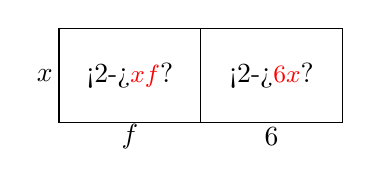
\begin{tikzpicture}[scale=0.6]

% Outer rectangle
\draw (0,0) rectangle (6,2);

% Vertical split
\draw (3,0) -- (3,2);

% Labels for widths
\node at (1.5,-0.3) {$f$};
\node at (4.5,-0.3) {$6$};

% Height label
\node at (-0.3,1) {$x$};

% Area labels
\node at (1.5,1) {\ashowq{$xf$}};
\node at (4.5,1) {\ashowq{$6x$}};

\end{tikzpicture}
    \par\vspace{0.5em}
    \ashow{Area = \(x(f+6)\)}
  \end{block}
\end{minipage}
\end{frame}
\begin{frame}<1>{Starter: Expand each expression}
% Option A: simple 2x2 grid using minipages (consistent spacing)
\begin{minipage}[t]{0.48\textwidth}
  \begin{block}{1) Single brackets}
    \Large \(\;3(y+5)=\ablank{3y+15}\)
  \end{block}
  \vspace{0.5em}
  \begin{block}{3) Double brackets}
    \Large \(\;(x+4)(x-2)=\ablank{x^2+2x-8}\)
  \end{block}
\end{minipage}\hfill
\begin{minipage}[t]{0.48\textwidth}
  \begin{block}{2) Single brackets}
    \Large \(\; a(b-5)=\ablank{ab-5a}\)
  \end{block}
  \vspace{0.5em}
  \begin{block}{4) What is the area of the rectangle?}
    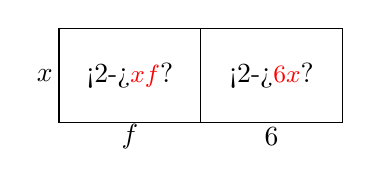
\begin{tikzpicture}[scale=0.6]

% Outer rectangle
\draw (0,0) rectangle (6,2);

% Vertical split
\draw (3,0) -- (3,2);

% Labels for widths
\node at (1.5,-0.3) {$f$};
\node at (4.5,-0.3) {$6$};

% Height label
\node at (-0.3,1) {$x$};

% Area labels
\node at (1.5,1) {\ashowq{$xf$}};
\node at (4.5,1) {\ashowq{$6x$}};

\end{tikzpicture}
    \par\vspace{0.5em}
    \ashow{Area = \(x(f+6)\)}
  \end{block}
\end{minipage}
\end{frame}
\begin{frame}<1>{Starter: Expand each expression}
% Option A: simple 2x2 grid using minipages (consistent spacing)
\begin{minipage}[t]{0.48\textwidth}
  \begin{block}{1) Single brackets}
    \Large \(\;3(y+5)=\ablank{3y+15}\)
  \end{block}
  \vspace{0.5em}
  \begin{block}{3) Double brackets}
    \Large \(\;(x+4)(x-2)=\ablank{x^2+2x-8}\)
  \end{block}
\end{minipage}\hfill
\begin{minipage}[t]{0.48\textwidth}
  \begin{block}{2) Single brackets}
    \Large \(\; a(b-5)=\ablank{ab-5a}\)
  \end{block}
  \vspace{0.5em}
  \begin{block}{4) What is the area of the rectangle?}
    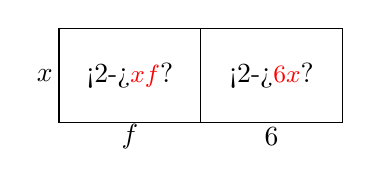
\begin{tikzpicture}[scale=0.6]

% Outer rectangle
\draw (0,0) rectangle (6,2);

% Vertical split
\draw (3,0) -- (3,2);

% Labels for widths
\node at (1.5,-0.3) {$f$};
\node at (4.5,-0.3) {$6$};

% Height label
\node at (-0.3,1) {$x$};

% Area labels
\node at (1.5,1) {\ashowq{$xf$}};
\node at (4.5,1) {\ashowq{$6x$}};

\end{tikzpicture}
    \par\vspace{0.5em}
    \ashow{Area = \(x(f+6)\)}
  \end{block}
\end{minipage}
\end{frame}
\begin{frame}<1>{Starter: Expand each expression}
% Option A: simple 2x2 grid using minipages (consistent spacing)
\begin{minipage}[t]{0.48\textwidth}
  \begin{block}{1) Single brackets}
    \Large \(\;3(y+5)=\ablank{3y+15}\)
  \end{block}
  \vspace{0.5em}
  \begin{block}{3) Double brackets}
    \Large \(\;(x+4)(x-2)=\ablank{x^2+2x-8}\)
  \end{block}
\end{minipage}\hfill
\begin{minipage}[t]{0.48\textwidth}
  \begin{block}{2) Single brackets}
    \Large \(\; a(b-5)=\ablank{ab-5a}\)
  \end{block}
  \vspace{0.5em}
  \begin{block}{4) What is the area of the rectangle?}
    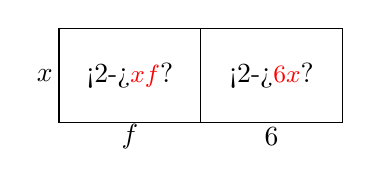
\begin{tikzpicture}[scale=0.6]

% Outer rectangle
\draw (0,0) rectangle (6,2);

% Vertical split
\draw (3,0) -- (3,2);

% Labels for widths
\node at (1.5,-0.3) {$f$};
\node at (4.5,-0.3) {$6$};

% Height label
\node at (-0.3,1) {$x$};

% Area labels
\node at (1.5,1) {\ashowq{$xf$}};
\node at (4.5,1) {\ashowq{$6x$}};

\end{tikzpicture}
    \par\vspace{0.5em}
    \ashow{Area = \(x(f+6)\)}
  \end{block}
\end{minipage}
\end{frame}

% ---------- ANSWERS ----------
\begin{frame}<1>{Answers}
\begin{enumerate}
  \item \(3(y+5)=3y+15\)
  \item \(a(b-5)=ab-5a\)
  \item \((x+4)(x-2)=x^2+2x-8\)
  \item Area = \(xf + 6x = x(f+6)\)
\end{enumerate}
\end{frame}
\begin{frame}<1>{Answers}
\begin{enumerate}
  \item \(3(y+5)=3y+15\)
  \item \(a(b-5)=ab-5a\)
  \item \((x+4)(x-2)=x^2+2x-8\)
  \item Area = \(xf + 6x = x(f+6)\)
\end{enumerate}
\end{frame}
\begin{frame}<1>{Answers}
\begin{enumerate}
  \item \(3(y+5)=3y+15\)
  \item \(a(b-5)=ab-5a\)
  \item \((x+4)(x-2)=x^2+2x-8\)
  \item Area = \(xf + 6x = x(f+6)\)
\end{enumerate}
\end{frame}
\begin{frame}<1>{Answers}
\begin{enumerate}
  \item \(3(y+5)=3y+15\)
  \item \(a(b-5)=ab-5a\)
  \item \((x+4)(x-2)=x^2+2x-8\)
  \item Area = \(xf + 6x = x(f+6)\)
\end{enumerate}
\end{frame}

% answer macro review note
\begin{frame}<1>
\frametitle{Automated check: answers may need attention}
The answers on these slides may have unresolved formatting issues. An automated
review did not accept them, and rewriting them did not settle it.

The review said the "final answers" frame and the "Answers" frame each show all answers on their first overlay, meaning nothing is hidden until a click. It doesn't name specific slides, only those two frame titles. The two comments are essentially the same complaint repeated, not contradictory, but it's worth checking whether showing all answers immediately is actually a mistake or an intentional design choice.

Please check these slides and either correct them or raise an issue.
\end{frame}
\begin{frame}<1>
\frametitle{Automated check: answers may need attention}
The answers on these slides may have unresolved formatting issues. An automated
review did not accept them, and rewriting them did not settle it.

The review said the "final answers" frame and the "Answers" frame each show all answers on their first overlay, meaning nothing is hidden until a click. It doesn't name specific slides, only those two frame titles. The two comments are essentially the same complaint repeated, not contradictory, but it's worth checking whether showing all answers immediately is actually a mistake or an intentional design choice.

Please check these slides and either correct them or raise an issue.
\end{frame}
\begin{frame}<1>
\frametitle{Automated check: answers may need attention}
The answers on these slides may have unresolved formatting issues. An automated
review did not accept them, and rewriting them did not settle it.

The review said the "final answers" frame and the "Answers" frame each show all answers on their first overlay, meaning nothing is hidden until a click. It doesn't name specific slides, only those two frame titles. The two comments are essentially the same complaint repeated, not contradictory, but it's worth checking whether showing all answers immediately is actually a mistake or an intentional design choice.

Please check these slides and either correct them or raise an issue.
\end{frame}
\begin{frame}<1>
\frametitle{Automated check: answers may need attention}
The answers on these slides may have unresolved formatting issues. An automated
review did not accept them, and rewriting them did not settle it.

The review said the "final answers" frame and the "Answers" frame each show all answers on their first overlay, meaning nothing is hidden until a click. It doesn't name specific slides, only those two frame titles. The two comments are essentially the same complaint repeated, not contradictory, but it's worth checking whether showing all answers immediately is actually a mistake or an intentional design choice.

Please check these slides and either correct them or raise an issue.
\end{frame}

\end{document}